% 2002 年春季上海卷第 10 题：正方体展开图
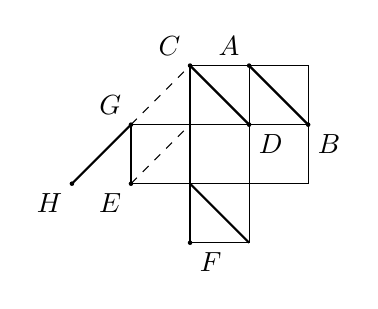
\begin{tikzpicture}[scale=0.75]
  \draw (0,0) rectangle (1,1);
  \draw (1,0) rectangle (2,1);
  \draw (2,0) rectangle (3,1);
  \draw (1,1) rectangle (2,2);
  \draw (2,1) rectangle (3,2);
  \draw (1,-1) rectangle (2,0);

  \draw[thick] (-1,0)--(0,1);
  \draw[thick] (1,2)--(2,1);
  \draw[thick] (2,2)--(3,1);
  \draw[thick] (1,0)--(2,-1);

  \draw[dashed] (0,1)--(1,2) (0,0)--(1,1);

  \fill (-1,0) circle (1.1pt) node[below left] {$H$};
  \fill (0,1) circle (1.1pt) node[above left] {$G$};
  \fill (0,0) circle (1.1pt) node[below left] {$E$};
  \fill (1,-1) circle (1.1pt) node[below right] {$F$};
  \fill (1,2) circle (1.1pt) node[above left] {$C$};
  \fill (2,1) circle (1.1pt) node[below right] {$D$};
  \fill (2,2) circle (1.1pt) node[above left] {$A$};
  \fill (3,1) circle (1.1pt) node[below right] {$B$};
\end{tikzpicture}
